\documentclass[11pt,a4paper]{scrartcl}

% Setup document
% Import Eidesstattliche Erklärung
\usepackage{pdfpages}
% Import graphics and wrap them
\usepackage{graphicx}
\usepackage{wrapfig}
\usepackage{float}

% Localization
\usepackage[utf8]{inputenc}
\usepackage[T1]{fontenc}
\usepackage[ngerman]{babel}

% Clickable table of contents
\usepackage{hyperref}
\usepackage[ngerman]{cleveref}

% Page formatting
\usepackage[automark]{scrlayer-scrpage}
\usepackage{typearea}
\usepackage{microtype}

% Better tables
\usepackage{tabularray}
\usepackage{booktabs}

% Develop Packages
\usepackage{blindtext}
% Variables
\newcommand{\vorname}{Lukas}
\newcommand{\nachname}{Szimtenings}
\newcommand{\matr}{Matr.-Nr.\ 3217694}
\newcommand{\uni}{FH Aachen}
\newcommand{\studiengang}{Angewandte Mathematik und Informatik}
\newcommand{\modul}{5. Semester 952006 (Aachen)}
\newcommand{\erstpruefer}{Alexander Voß}
\newcommand{\zweitpruefer}{Raphael Majeed}
\newcommand{\subtitel}{ Verteilte Ausführung von in konjunktiver Normalform spezifizierten Machbarkeitsabfragen in medizinischen Datenintegrationszentren }
\newcommand{\titel}{- Seminararbeit -}
\newcommand{\location}{Aachen}
\newcommand{\abteilung}{Abteilung: Research Infrastructure}
\newcommand{\abteilungabkuerzung}{RI}

%images
\newcommand{\uklogo}{
    
\includegraphics[scale=0.5]{res/logo-uniklinik-rwth-aachen}
    
\includegraphics[scale=0.6]{res/imi_sublogo}
}

\newcommand{\ukimilogo}{
\includegraphics[scale=0.16]{res/imilogo}}
% command for wrapfigure -> more than one figure per paragraph
\newcommand*{\invisiblepar}{{\setlength{\parfillskip}{0pt}\par}\vskip-\parskip\noindent\ignorespaces}
% Metadata
\title{\titel}
\author{\vorname{} \nachname}
\date{\today{}, \location}

% Pagestructure
\clearpairofpagestyles
%footer
\ifoot[]{\ukimilogo}
\cfoot[]{\abteilungabkuerzung}
\ofoot[]{\pagemark}
%header
\ihead[]{\vorname\ \nachname}
\chead[]{\titel}
\ohead[]{\matr}
%Seperator
\setheadsepline[\textwidth]{1pt}
\setfootsepline[\textwidth]{1pt}

\begin{document}
%% Prefix %%
% Titelblatt
\begin{titlepage}
    \centering
    {\scshape\LARGE \uni{} \par \studiengang{} \par \modul{} \par}
    \vspace{1cm}
    {\scshape\Large \titel{} \par}
    \vspace{1.5cm}
    {\bfseries \huge \subtitel{} \par}
    \vspace{2cm}
    {\Large \vorname{} \nachname{} \par \matr{} \par}
    \vfill
    \begin{center}
        \itclogo{}
        \par
        \abteilung{}
    \end{center}

    \par\vfill
    \parbox{4cm}{\hrule \strut{} \centering \footnotesize \vorname{} \nachname{} \par \textit{Autor}}
    \hfill
    \parbox{5cm}{\hrule \strut{} \centering \footnotesize \erstpruefer{} \par \textit{Erstprüfer}}
    \hfill
    \parbox{4cm}{\hrule \strut{} \centering \footnotesize \zweitpruefer{} \par \textit{Zweitprüfer}}
    \vfill
    {\large \location{} \today \par}
\end{titlepage}
% Einbinden der Eidesstattlichen Erklärung
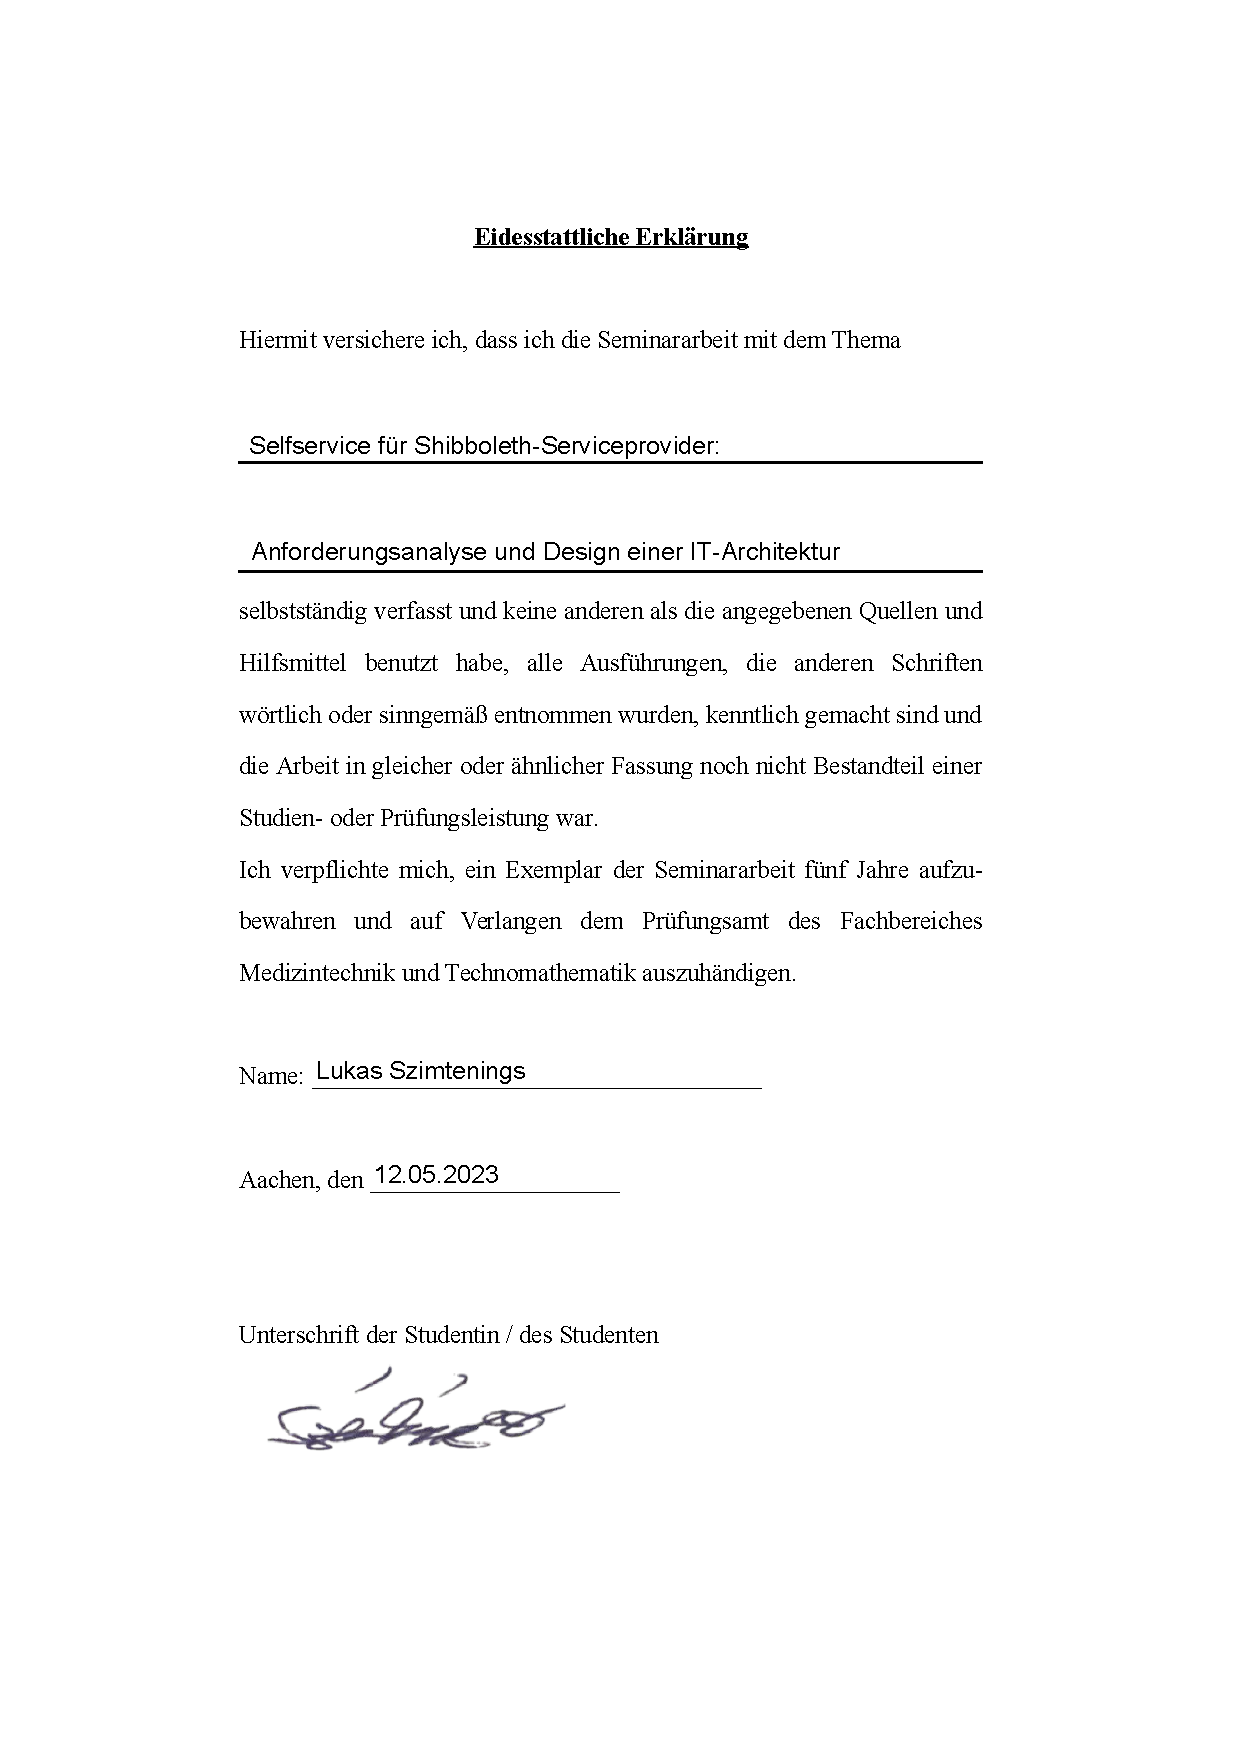
\includepdf{res/EidesstattlicheErklaerung.pdf}
\tableofcontents
\newpage

%% Hauptteil %%
% Seitenzahlen beginnen ab hier
\pagenumbering{arabic}

\section{Einführung}\label{sec:einfuehrung}
   \subsection{Problemstellung}\label{subsec:problemstellung}
   \subsection{Zielsetzung}\label{subsec:zielsetzung}
   \subsection{Abgrenzung}\label{subsec:abgrenzung}

\section{Grundlagen}\label{sec:grundlagen}
   \subsection{Single Sign-On (SSO)}\label{subsec:sso}
   \subsection{Shibboleth}\label{subsec:shibboleth}
      \subsubsection{Service Provider}\label{subsubsec:shib-sp}
      \subsubsection{Identity Provider}\label{subsubsec:shib-idp}
      \subsubsection{Metadaten}\label{subsubsec:shib-metadata}

\section{Stakeholder-Analyse}\label{sec:stakeholder}
   \subsection{Serviceprovider}\label{subsec:serviceprovider}
   \subsection{IT-Center}\label{subsec:itcenter}
   \subsection{Endnutzer}\label{subsec:endnutzer}
   \subsection{Stakeholder-Interessen und -Anforderungen}\label{subsec:stakeholder-anforderungen}

\section{Anforderungsanalyse}\label{sec:anforderungen}
   \subsection{Funktionale Anforderungen}\label{subsec:funktionale-anforderungen}
      \subsubsection{Beschreibung der Anforderungen}\label{subsubsec:beschreibung}
      \subsubsection{Priorisierung der Anforderungen}\label{subsubsec:priorisierung}
      \subsubsection{Abhängigkeiten zwischen den Anforderungen}\label{subsubsec:abhaengigkeiten}
   \subsection{Nicht-funktionale Anforderungen}\label{subsec:nicht-funktionale-anforderungen}
      \subsubsection{Sicherheitsanforderungen}\label{subsubsec:sicherheit}
      \subsubsection{Benutzerfreundlichkeitsanforderungen}\label{subsubsec:benutzerfreundlichkeit}
      \subsubsection{Kompatibilitätsanforderungen}\label{subsubsec:kompatibilitaet}

\section{Konzeption des Selfservice-Portals}\label{sec:konzeption}
   \subsection{Entwurf der Benutzeroberfläche}\label{subsec:entwurf}
   \subsection{Auswahl der technischen Plattform}\label{subsec:auswahl}
   \subsection{Integration mit dem Shibboleth-System}\label{subsec:integration}
   \subsection{Umsetzung des Selfservice-Portals}\label{subsec:umsetzung}

\section{Zusammenfassung und Ausblick}\label{sec:zusammenfassung}
   \subsection{Zusammenfassung der Ergebnisse}\label{subsec:zusammenfassung}


%% Suffix %%
\newpage

% Bibliographie
\pagenumbering{Roman}
\bibliography{Seminararbeit}
\bibliographystyle{unsrt}

% Abbildungsverzeichnis
\listoffigures
\end{document}